\begin{frame}{Overview}
\section{Implementation}
The model contain two main parts
\begin{itemize}
    \item Training Environment
    \item RL Model. 
\end{itemize}
\begin{center}
  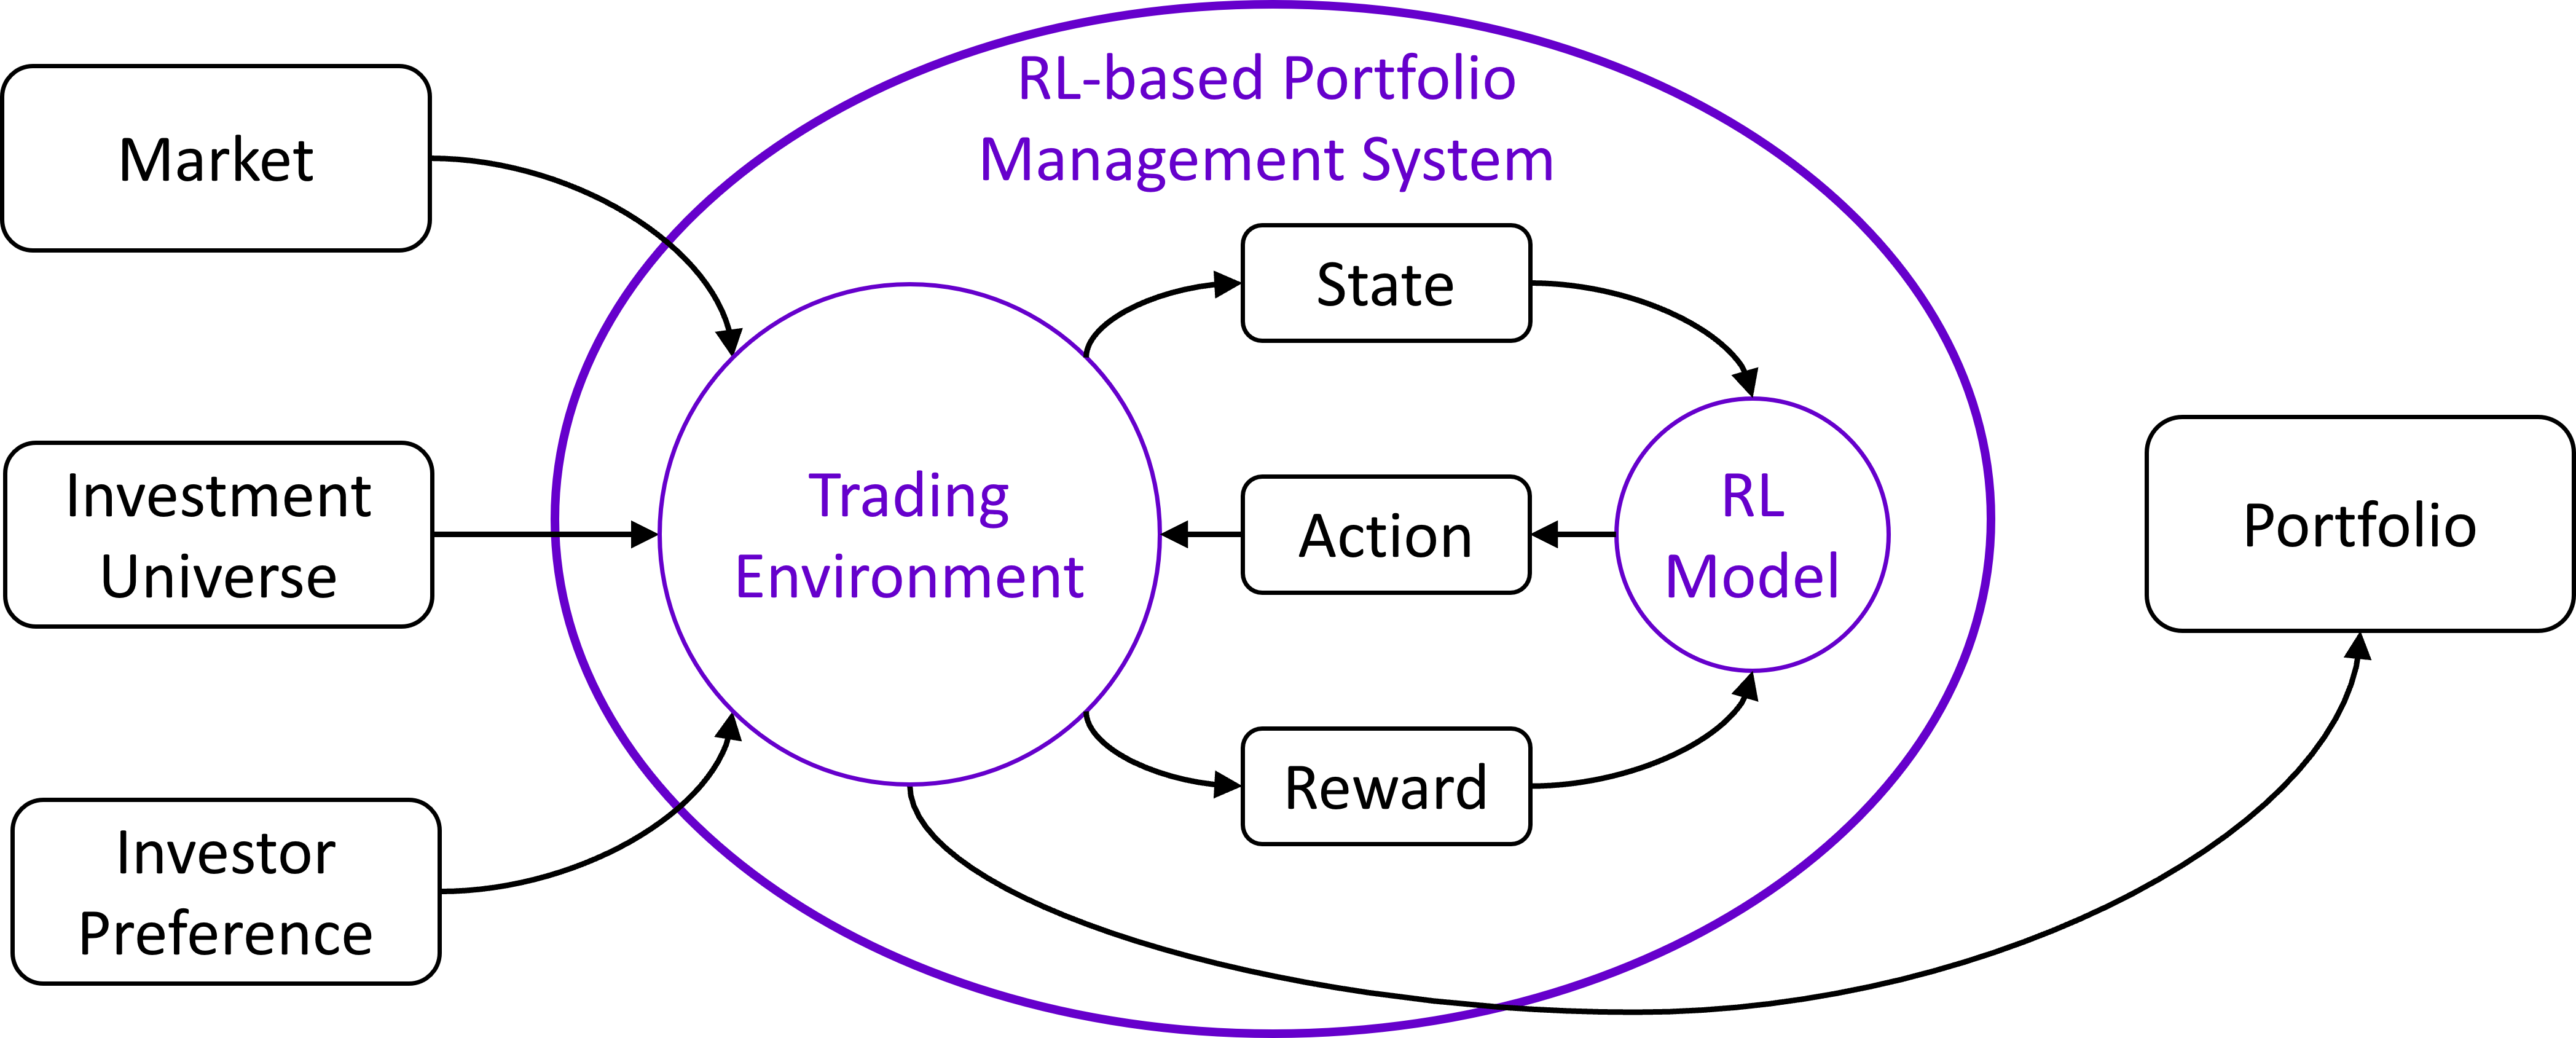
\includegraphics[width=10cm]{images/context_diagram.png}  
\end{center}
\end{frame}



\begin{frame}{Investment Universe}
\end{frame}


\begin{frame}{Market Features}
Structured information from the market as its data source, including interest rates, commodity prices and currency exchange indexes.
For stationary data, we will use them directly as features. For non-stationary data, we use statistics measures among 5, 20, and 60 days as features, including standard deviation, skewness, and kurtosis.
\end{frame}



\begin{frame}{Investor Preference}
Risk aversion of the investors. 
Acquire risk aversion
Professional personnel or organization will acquire risk aversion from investors by survey or other techniques and interprets the inputs into comparable indicators between investors.

MDD as be 

\begin{block}{MDD}
One of the indicators to evaluate our system. However, optimizing any ratio using MDD directly has many problems and challenges. Some researches indicate MDDs are outliers or imply optimizing MDD is troublesome. Therefore, we will limit ourselves to use MDD while optimizing the model and consider other alternatives. 
\end{block}
\end{frame}



\begin{frame}{Reinforcement Learning Model}
\begin{block}{Overview}
Soft Actor-Critic (SAC) is an DRL algorithm that optimizes a stochastic policy in an off-policy way.
Unlike other RL models, which usually optimize the expected return, SAC optimizes the policy with entropy regularization and takes entropy, measuring randomness in the policy, into account.
\end{block}
\begin{block}{Reward Scale}
SAC is highly sensitive to the scaling of the reward. If the reward scale is too small, the reward will fail to affect the model, and the policy will become nearly uniform. The model will learn quickly and become deterministic for reward scale too large, leaving no room for exploration.
\end{block}
\end{frame}



\begin{frame}{Trading Environment}
A trading environment compatible with Open AI Gym
\begin{center}
  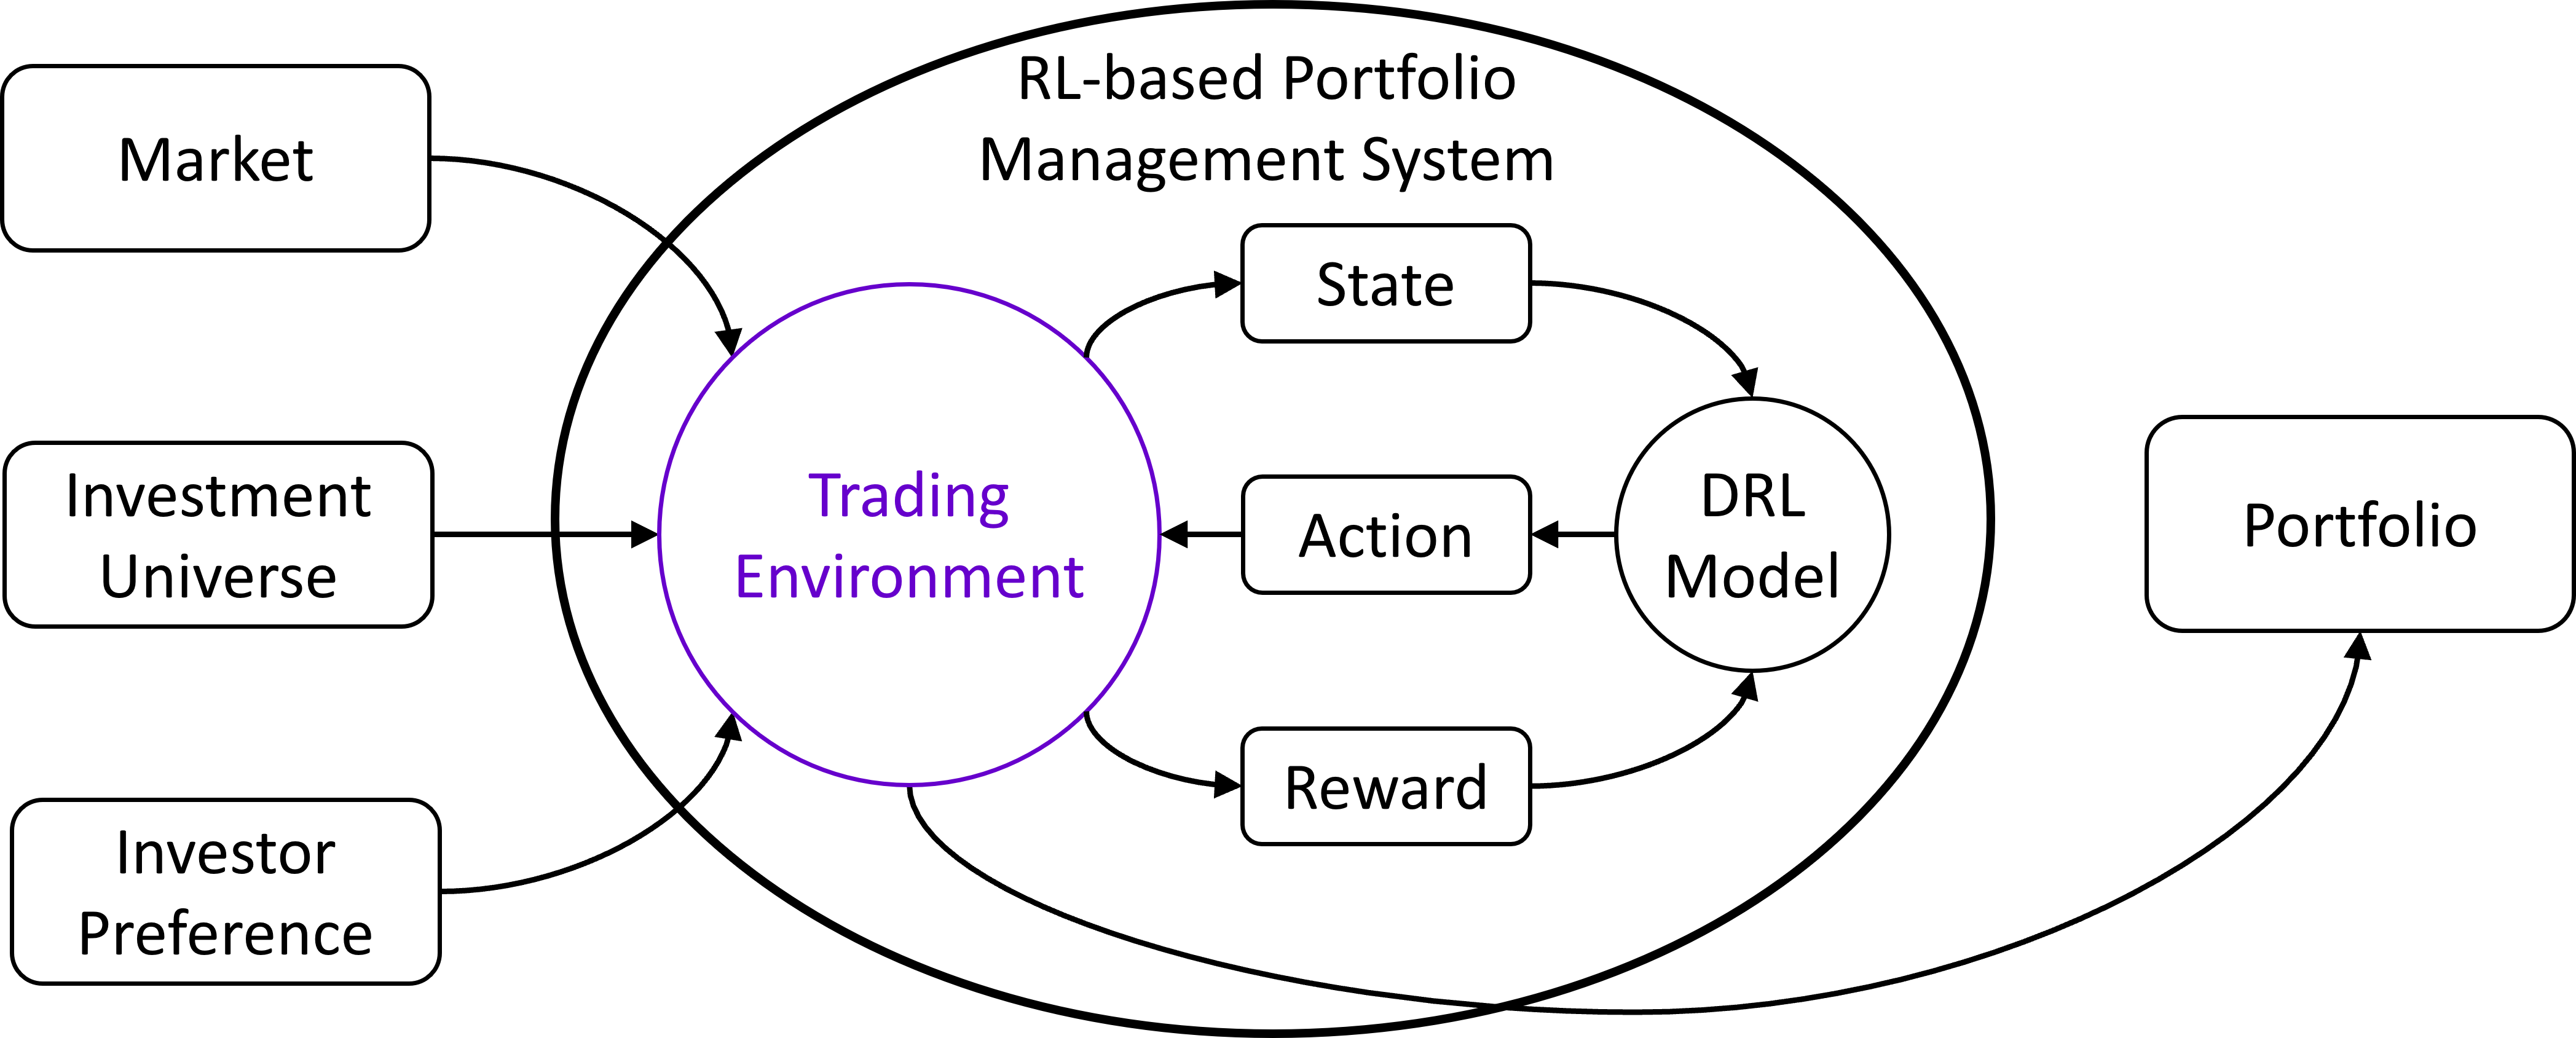
\includegraphics[width=10cm]{images/trading_environment.png}
\end{center}
\end{frame}

\begin{frame}{Feature Extractor}
\begin{center}
  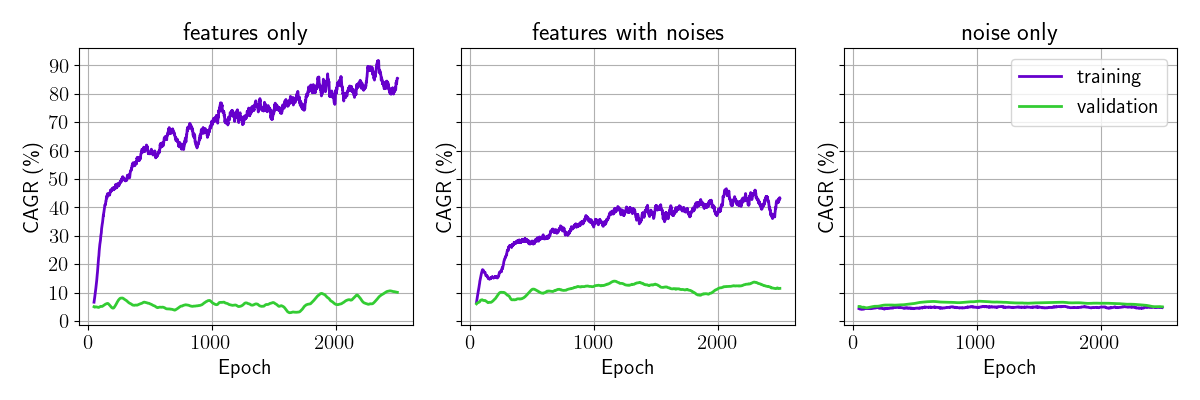
\includegraphics[width=10cm]{images/compare_noise.png}
\end{center}
\end{frame}

\begin{frame}{Portfolio Builder}
The portfolio builder builds the portfolio from the investible universe and the action from the RL model.
The portfolio F contains no short position and is an m dimension vector space of weights w, a real number between 0 and 1. , where m is the number of investments in the investment universe. Wealth will all be in the form of investments, so the sum of the weights will equal 1.
\[
    F = \{ {f \in \mathbb{R} | 0 \leq f \leq 1 } \} ^m,
    \sum_{i=1}^m {f_i} =1
\]
We distribute the weight based on the action proportionally.
\[
    F_i = \cfrac{a_i}{\sum a} 
\]
where \(F_i\) is the weight for \(i^{th}\) investment, \(a_i\) is the  \(i^{th}\) action, m is the total number of investments in the investible universe. 

\end{frame}


\begin{frame}{Trading System}
The trading system measures performances of the given portfolios, including MDD, CAGR, profit, and wealth. These performances will be the input to calculate the reward or evaluate the performance of the system. 
    
\end{frame}

\begin{frame}{Reward Provider}
We first use profit p as the baseline for the reward and add a penalty, \(p_t-\theta\), upon negative profits exceeding the given absolute value threshold \(\theta\). 
\[
p_t = \frac{w_t-w_{t-1}}{w_{t-1}}
, 
R_t = 
\begin{cases}
    p_t,&\text{if  }p_t > -\theta\\
    2p_t - \theta ,&\text{if  }p_t \leq  \theta
\end{cases}
\]
where \(R_t\) is the reward, \(p_t\) is the profit and \(w_t\) is the wealth on given t.
\\
On all threshold \(\theta\) given, the result shows unstable improvement in MDD. We observed that the optimization goes too well during training and generates a tiny amount of negative profits; therefore, these negative profits have minimal penalty effect on the model parameters.
\\

\end{frame}

\begin{frame}{Reward Provider}
We then apply the penalty upon both positive and negative profits. This increases the stability significantly.
\[
R_t = 
\begin{cases}
    2p_t - \theta,&\text{if  }    $$|p_t|$$ > \theta\\
    p_t - \theta ,&\text{if  } $$|p_t|$$\leq  \theta
\end{cases}
\]
The threshold \(\theta\) will be the main adjustable parameter of our system. Adjusting it will enable the system to produce portfolios to meet different investors' risk tolerance.
\end{frame}
\begin{frame}{Reward Provider}
\begin{center}
      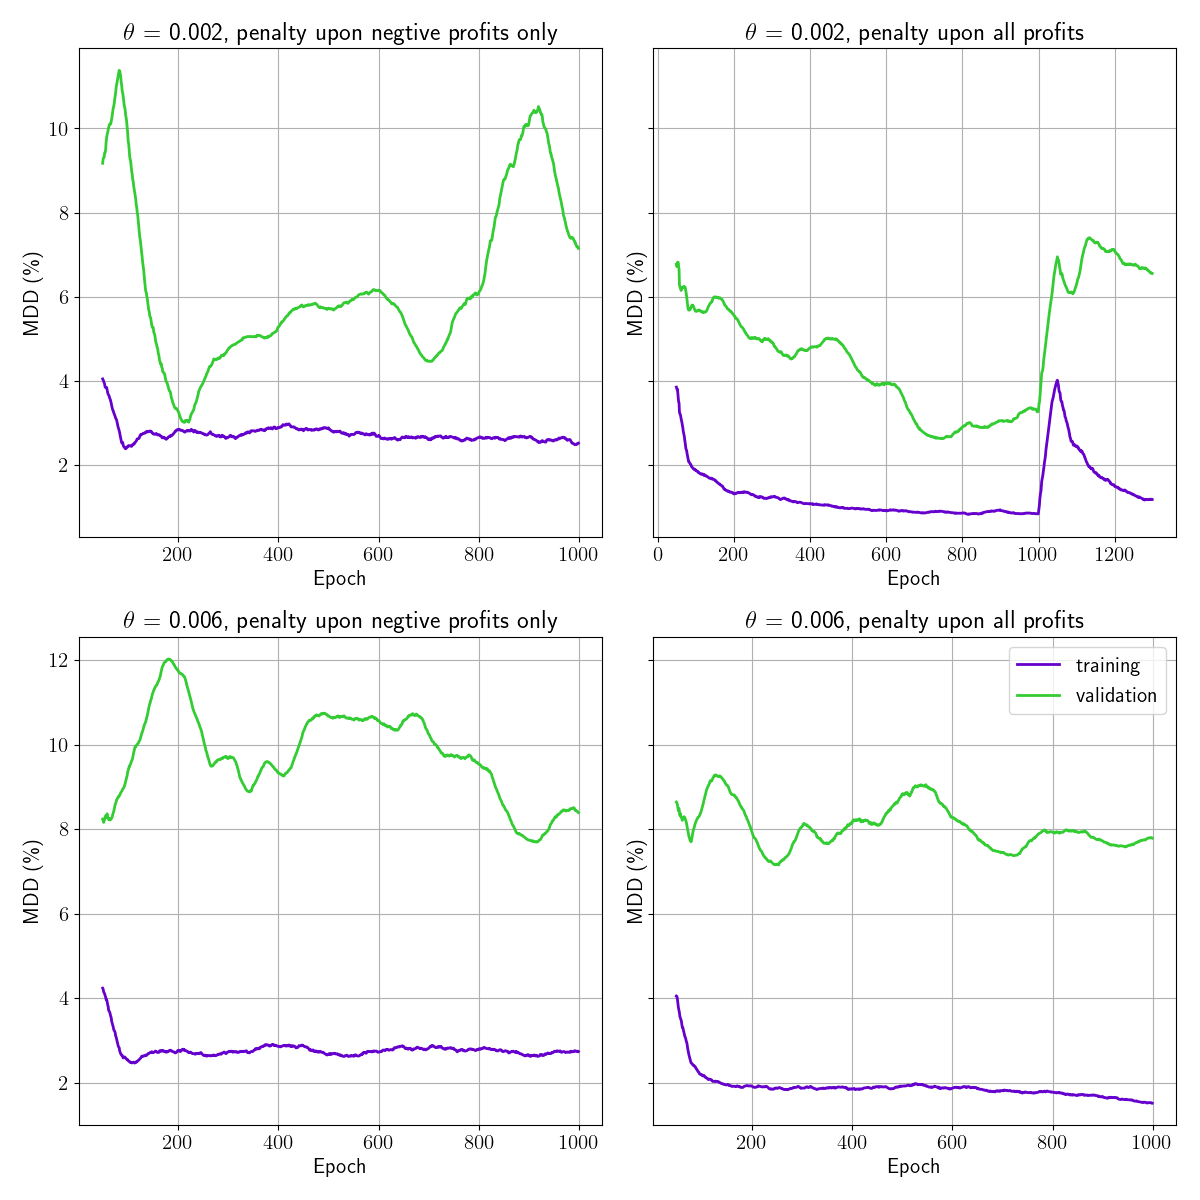
\includegraphics[height=7cm]{images/penalty_negtive_profits_compare.png}
\end{center}
\end{frame}

\begin{frame}{Result}
\begin{center}
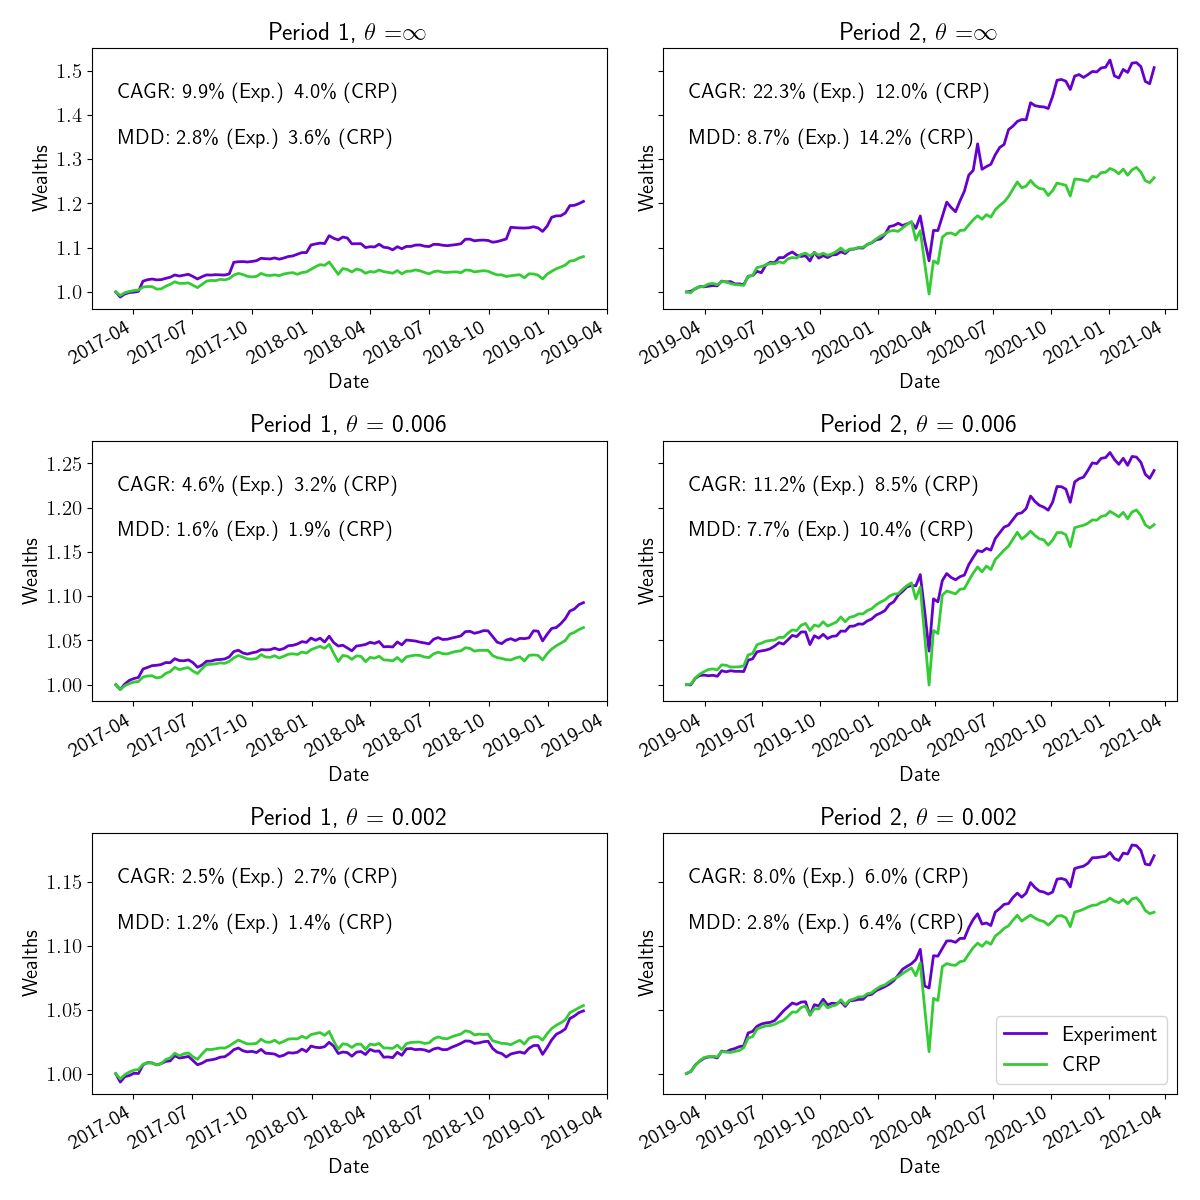
\includegraphics[height= 7.5cm]{images/crp_compare.png}
\end{center}
\end{frame}
